\documentclass[11pt,a4paper,leqno]{article}
\usepackage{a4wide}
\usepackage[T1]{fontenc}
\usepackage[utf8]{inputenc}
\usepackage{amsmath, amssymb, amsfonts, amsthm, bm, delarray}
\usepackage{caption}
\usepackage{listings}
\usepackage{parskip}
\usepackage[unicode=true]{hyperref}
\hypersetup{colorlinks=true, linkcolor=black, anchorcolor=black, citecolor=black, filecolor=black, menucolor=black, runcolor=black, urlcolor=black}
\setlength{\parskip}{.5ex}
\setlength{\parindent}{0ex}

\theoremstyle{definition}
\newtheorem{exercise}{Exercise}
\renewcommand{\theenumi}{\roman{enumi}}

\usepackage{graphicx}
\graphicspath{ {./images/} }

\begin{document}

    \begin{center}
        \begin{large}
            \textbf{
                Vocabulary and Translation GUI\\
                Effective Programming Practices for Economists\\
                Universität Bonn, Winter 2022/22\\[2ex]
                Ayse Irem Yilmaz\\}
        \end{large}
    \end{center}
    
    \begin{center}
        Click \href{https://github.com/irem-y/vocabulary_and_translation_gui}{\textcolor{blue}{here}} to view the project.\\
        Submission: 29.03.2023
    \end{center}
    
    \newpage

    \tableofcontents

    \newpage
    
    \section{Introduction}
    My project is graphical user interface to help me to improve my language skills, especially to learn and memorize more vocabulary.\\\\
    The program can use the languages English, German and Turkish.
    I chose these languages because my native language is Turkish and I want to improve my German and English.\\\\
    To create the GUI I use the package \emph{Tkinter}.
    To translate words and phrases I use the \href{https://github.com/DeepLcom/deepl-python}{\textcolor{blue}{DeepL API}}.
    To check the spelling of words and phrases I use the spellchecking library \emph{PyEnchant}.
    Finally, to save the vocabulary as an Excel file, I used the \emph{openpyxl} package, and as an Anki file, the \emph{genanki} package.
    
    \newpage
    
    \section{Usage}
    To see how to set up and use the program in detail, read the \emph{README.md} file.\\
    Here is a picture of the GUI:\@
    \begin{figure}[h]
        \caption{Graphical User Interface}
        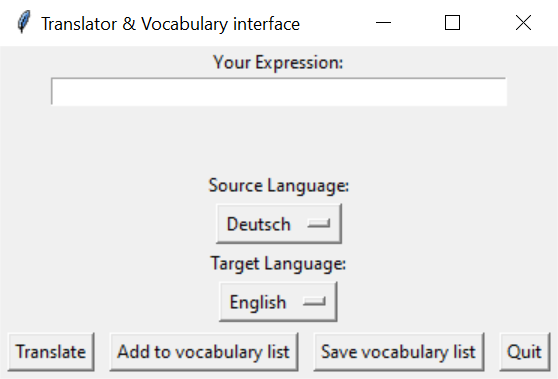
\includegraphics{GUI_screenshot.PNG}
    \end{figure}\\  
    The GUI allows you to translate words directly using the \emph{'Translate'} button, or add them to a list using the the \emph{'Add to vocabulary list'} button.
    The list can then be saved using the \emph{'Save vocabulary list'} button.
    The user can then choose where to save the file and in what format, as an Excel or Anki file.
    
    \newpage

    \section{Pytask}

    I have created five tasks:
    \begin{enumerate}
        \item task\_get\_key: This task checks if in the given file a DeepL key is available.
        \item task\_check\_dictionaries: This task checks if all required dictionaries are available.
        \item task\_compile\_latex\_document: This task compiles the LaTex documentation file and creates a PDF.
        \item task\_test\_all\_functions: This task performs a unit test for all funcitons wit pytest.
        \item task\_create\_user\_interface: This task checks if the user interface can be created.
    \end{enumerate}

    \newpage

    \section{Remarks}
    
    I have written and tested the code on Microsoft Windows 10. Other operating systems may cause problems.\\\\
    I needed to add German and Turkish dictionaries to the \emph{enchant} library to be able to spell check words in those languages.
    The program checks to see if all the required dictionaries are available, and guides the user through the steps to add them if necessary.

\end{document}
